\documentclass[12pt]{article}

\usepackage[hmargin=1in, vmargin=1in]{geometry}
\usepackage{bm}
\usepackage{booktabs}
\usepackage{amsmath}
\usepackage{mathtools} 
\usepackage{graphicx}
\usepackage{soul}
\usepackage{color}
\usepackage[dvipsnames]{xcolor}
\usepackage[section]{placeins}
\usepackage{natbib}
\bibliographystyle{plainnat}
%\bibliographystyle{ecol_let}   %% RC: I also added ecology.bst
\setcitestyle{round}
\usepackage{booktabs}
\usepackage{amssymb}
\usepackage[backgroundcolor=white]{todonotes}
\pagestyle{myheadings}
\markright{A Joint Likelihood Alternative to WAIC}

\DeclarePairedDelimiter\Floor\lfloor\rfloor
\DeclarePairedDelimiter\Ceil\lceil\rceil
\DeclarePairedDelimiter\abs{\lvert}{\rvert}
\DeclarePairedDelimiter\norm{\lVert}{\rVert}

\newcommand{\bs}{{\bm s}}
\newcommand{\cS}{{\mathcal S}}
\newcommand{\ds}{{\, \mathrm{d} \bm s}}
\newcommand{\Bern}{{\mathrm{Bern}}}
\newcommand{\Bin}{{\mathrm{Bin}}}
\newcommand{\Po}{{\mathrm{Pois}}}
\newcommand{\Gam}{{\mathrm{Gamma}}}

% comment command, wrapping \todo[inline]{}
\newcommand{\cmt}[1]{\todo[inline]{\color{blue} #1}}

\DeclareRobustCommand{\hlrc}[1]{{\sethlcolor{Dandelion}\hl{#1}}}


\title{A Joint Likelihood Alternative to WAIC for N-Mixture Models}
\author{Heather Gaya and Friends}
\date{2020}
\begin{document}
\maketitle

\section{Introduction}

Model selection is a critical part of analyzing ecological data. Often the importance of covariates for predicting a system is unknown and there is no available information on the most important variables in an ecological system. To further complicate the issue, observations are often biased by imperfect detection and human error, so direct data on the system is unavailable. To confront these challenges, a suitable method is needed to evaluate and compare available candidate models. While multiple methods have been proposed and thoroughly tested under a maximum likelihood framework, comparatively few methods have been discussed for a Bayesian framework and no consensus has been reached on which is the best option. 

One popular method of Bayesian model selection is 	WAIC \citep{Watanabe_2010}, a generalized version of AIC for Bayesian models. WAIC combines the estimated log predictive density of the data with a penalty for the estimated number of parameters in the model to produce a value that can be compared between alternative models. This method is valid in both hierarchical and mixture models \citep{Watanabe_2010} and has been shown to be an efficient alternative to cross-validation \citep{Gelman_2014}. However, WAIC may fail when data are correlated (such as spatial or temporal models) \citep{Hooten_2015, Link_2020}. 


\section{Methods}

\subsection{WAIC}
 WAIC \citep{Watanabe_2010} estimates the expected log predictive densities for all data points and is defined as:
 \begin{gather*}
 WAIC = -2\widehat{lpd} + 2\widehat{p}_{waic}
 \end{gather*}
 where $\widehat{lpd}$ is the log predictive density of the data:
   \begin{gather*}
  lpd = \sum_{i = 1}^{n} log(P(y_i | \theta_i))
  \end{gather*}
  and $\widehat{p}_{waic}$ is the estimated effective number of parameters:
    \begin{gather*}
  p_{waic} = \sum_{i = 1}^{n} var_{post}(log(P(y_i | \theta_i))
  \end{gather*} 
 
 If $y_i$ and $\theta$ are directly linked, and there is no error in the data, then WAIC is likely sufficient for finding the top model. However, in many wildlife models, error is introduced into the data in the form of imperfect detection. Consider a simple Binomial $N$-mixture model where both abundance, $N$, and detection probability, $p$, vary with site $i$. 
 \begin{gather*}
    \mathrm{log}(\lambda_i) = \beta_0 + \beta_1  x_{i1} +
    \beta_2 x_{i2} + \cdots \\
    N_i \sim \mathrm{Poisson}(\lambda_i)\\
    \mathrm{logit}(p_{ij}) = \alpha_0 + \alpha_1 x_{i1} + \cdots \\
    y_{ij} \sim \mathrm{Binomial}(N_i, p_{ij})
  \end{gather*}
  
WAIC only considers the fit of the data $y_{ij}$ to the latent abundance $N_i$ as it relates to $p_{ij}$. As $p_{ij}$ approaches 1, the log predictive density of the data approaches 0. 

%1^y(0)^N_i -y = 1

 \begin{gather*}
 P(y_{ij}| p_{ij}, N_{i}) = p_{ij}^{y_{ij}}(1-p_{ij})^{(N_i-y_{ij})} \\
\lim_{p_{ij} \to 1} log(P(y_{ij}| p_{ij}, N_{i})) = 0
 \end{gather*}
 
Therefore, as $p_{ij}$ approaches 1, the state process model has no effect on WAIC. 

Similarly, as $p_{ij}$ approaches 0:
 %0^1*(1-0)^(N_i-y) = 1 
 \begin{gather*}
 P(y_{ij}| p_{ij}, N_{i}) = p_{ij}^{y_{ij}}(1-p_{ij})^{(N_i-y_{ij})} \\
 \lim_{p_{ij} \to 0} log(P(y_{ij}| p_{ij}, N_{i})) = 0
 \end{gather*}


This heavily constrains situations where the use of WAIC is appropriate. 

 
\subsection{WAICj}
We suggest an adjustment to WAIC that considers the joint-likelihood of the data and relevant latent variables. We define our joint-likelihood approach to WAIC as:
\begin{gather*}
 WAIC = -2\widehat{jlpd} + 2\widehat{p}_{waicj}
 \end{gather*}
 with:
   \begin{gather*}
  jlpd = \sum_{i = 1}^{n} log(P(y_i | N_i)) + log(P(N_i | \lambda_i)) \\
  p_{waicj} = \sum_{i = 1}^{n} var_{post}(log(P(y_i | N_i)) + log(P(N_i | \lambda_i)))
  \end{gather*} 
Under this formulation, model selection will account for the log likelihood in both the detection model and the underlying state process model. 

\subsection{Marginalized N}

An alternative approach is to marginalize N in the model. 

\subsection{Simulated Case Study}

To test our WAIC approaches, we simulated 300 bird abundance data sets at 50 sites from a poisson distribution. We simulated detection as four independent visits of each site with a negative effect of windspeed on detection probability. The covariate coefficients for the  the detection and state process models were drawn randomly for each simulation. We further tested the effect of different sample sizes (15, 25, and 50 sites) and detection functions (low detection and high detection) on WAIC performance.  We analyzed each simulation's data using 4 candidate binomial N-mixture models (Table ~\ref{table:CandidateMods}) and used all three formulations of WAIC to assess model performance. 

\section{Results}
Across all simulations, WAIC correctly identified the top model in  67.5\%, 81.2\%, and 73.2\% of simulations under the traditional, joint-likelihood, and marginalization approaches respectively. The joint-likelihood approach tended to rank the correct model as the top model more often than the other two methods (Figure ~\ref{fig:modranks}).  All three metrics had more accurate model selection and gave more weight to the correct model when detection was lower and sample size was highest ~\ref{table:modweights})


\section{Discussion}
WAICj is better but it's still not perfect. Oof. 

\section{Literature Cited}
\bibliography{WAICj.bib}

\newpage

\begin{table}
\begin{center}
\begin{tabular}{ll} 

Model Number &  Formulation \\ 
  \hline
 Model 1* & $\lambda(tree_i)p(wind_{it})$ \\ 
 Model 2 & $\lambda(.)p(.)$ \\ 
 Model 3 & $\lambda(tree_i)p(.)$ \\ 
 Model 4 & $\lambda(.)p(wind_{it})$ \\ 
 \hline
\end{tabular}
\caption{Candidate Models. The asterisk denotes the model under which data was simulated. Periods represent intercept only models.}
\label{table:CandidateMods}
\end{center}
\end{table}

\newpage

\begin{table}
\begin{center}
\begin{tabular}{lcccccc} 
 \hline
 &  \multicolumn{3}{c}{Low Detection} &  \multicolumn{3}{c}{High Detection} \\
  \hline
  No. Sites & WAIC & WAICj & Marginalized & WAIC & WAICj & Marginalized\\ 
 \hline
 15 & 0.59 (.27) & .69 (.31) & .57 (.31) & .57 (.32) & .74 (.33) & .73 (.30)\\
 25 & 0.66 (.30) & .79 (.28) & .67 (.33) & .66 (.32) & .85 (.26) & .82 (.29)\\
 50 & 0.77 (.27) & .83 (.29) & .75 (.30) & .60 (.34) & .86 (.27) & .85 (.26)\\ 
\end{tabular}
\caption{Weight Given to the Correct Candidate Model. Each site and detection combination represents the mean (sd) weight from 100 simulations.}
\label{table:modweights}
\end{center}
\end{table}

\newpage

\begin{center}
\begin{figure}
  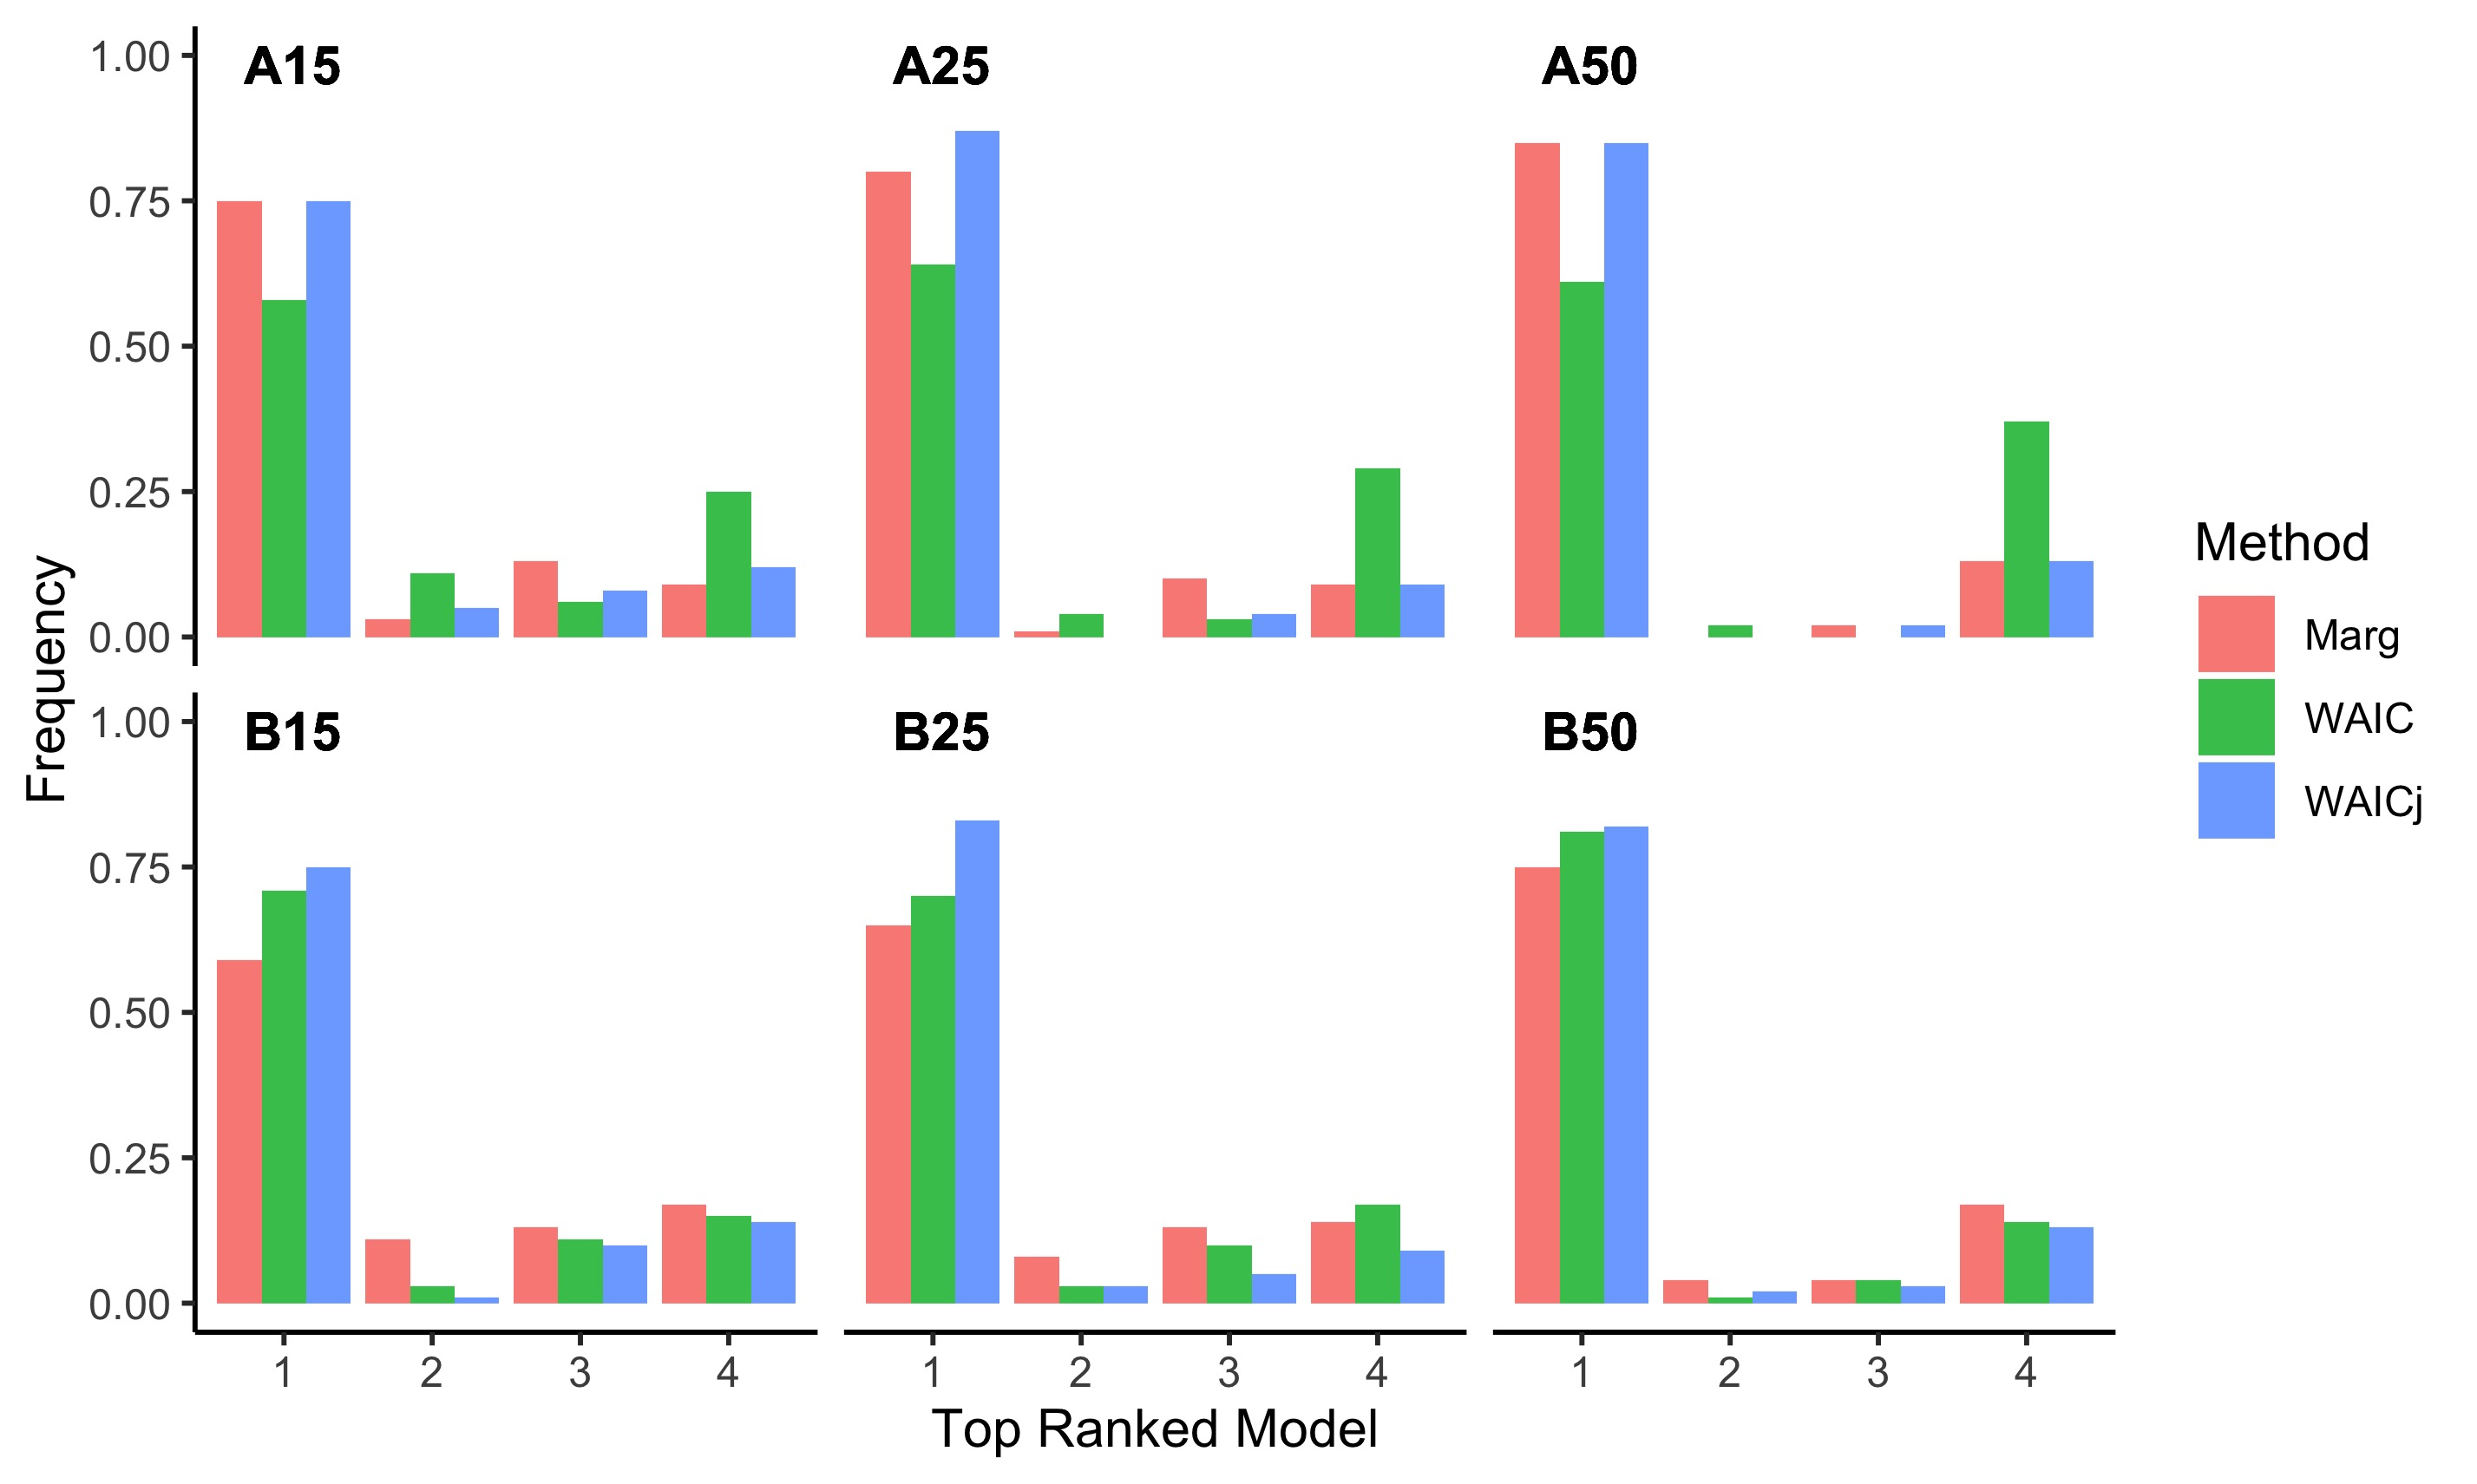
\includegraphics[scale=.15]{Ranking_WAIC.jpeg}
  \caption{Model Ranking Under a A. High Detection and B. Low Detection Scenario. Each scenario was analyzed with data from 15, 25 and 50 sites.}
  \label{fig:modranks}
\end{figure}
\end{center}



 
 
 \end{document}
  